This section details the categorization of signal events and the background estimation for the \wh{} analysis.

The \wh{} analysis requires exactly three isolated leptons (muons or electrons, including those from leptonic $\tau$ decays) with $\pt{} > 15$ GeV and total charge $\pm{e}$, with at least one being matched to the triggering lepton with $\pt{} > 27$ GeV. These requirements target backgrounds that could arise from multiple misidentified leptons, originating from $W+$jets production or $b\bar{b}$ production, and makes them negligible.

When the Higgs bosons decay into two $W$ bosons, the opening angle between the two resulting leptons is small compared to the angle between either of them and the lepton originating from the decay of the associated vector boson, due to helicity conservation and the V-A nature of the weak interaction. Due to this topology, a lepton labeling scheme is developed where the leptons are classified by identifying \lzero{} as the lepton with unique charge, \lone{} as the lepton closest in $\Delta{R}$ to \lzero{}, and \ltwo{} as the remaining lepton. The \lzero{} lepton is guaranteed to be from the Higgs boson decay due to the charge requirement of $\pm{e}$, and \lone{} is also likely from the Higgs boson decay due to spin correlations. Previously, it has been verified with MC simulation that \lzero{} is chosen correctly 99\% of the time, and \lone{} 85\% of the time for signal events. The labeling scheme is illustrated in Figure~\ref{fig:vh_wh_feynmann_diagram}.

\begin{figure}[htp]
    \centering
    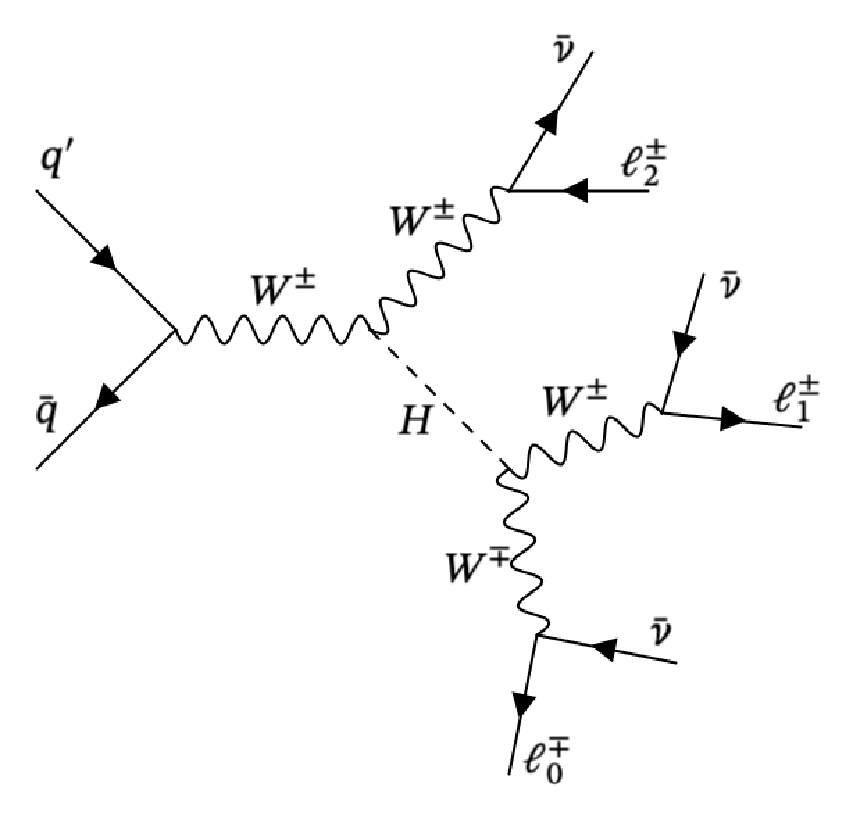
\includegraphics[width=0.5\textwidth]{
        figures/VH/VH_wh_feynmann.pdf
    }
    \caption{\wh{} Feynman diagram with corresponding lepton labeling shown.}\label{fig:vh_wh_feynmann_diagram}
\end{figure}

In order to separate regions populated with backgrounds from $Z$ bosons, such as $WZ/W\gamma^{*}$, $ZZ^{*}$, and $Z\gamma{}$, the analysis separates events with at least one SFOS lepton pair from those with none. The region with these pairs contains about 3/4 of the signal, but suffers from this irreducible background. The pair without any SFOS pair contains 1/4 of the signal, but needs stringent lepton identification to reduce backgrounds. Events containing at least one SFOS pair are classified as being in the \zdom{} category, while those without any in the \zdep{} category. The Feynman diagrams for the two leading prompt lepton backgrounds are presented in Figure~\ref{fig:vh_wh_leading_prompt_bkg}.

\begin{figure}[htp]
    \centering
    \subfloat[$q\bar{q} \to WZ$]{
        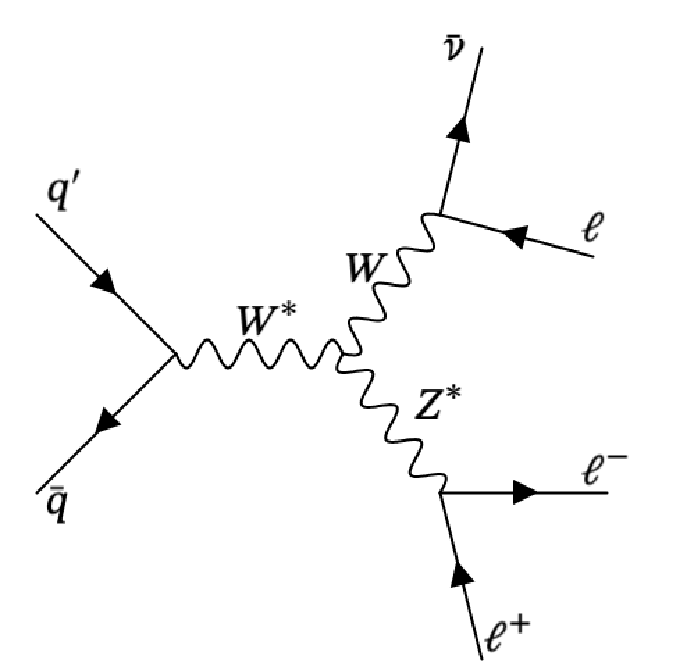
\includegraphics[width=0.4\textwidth]{figures/VH/qq_wz1.pdf}
    }
    \subfloat[$q\bar{q}\to ZZ$]{
        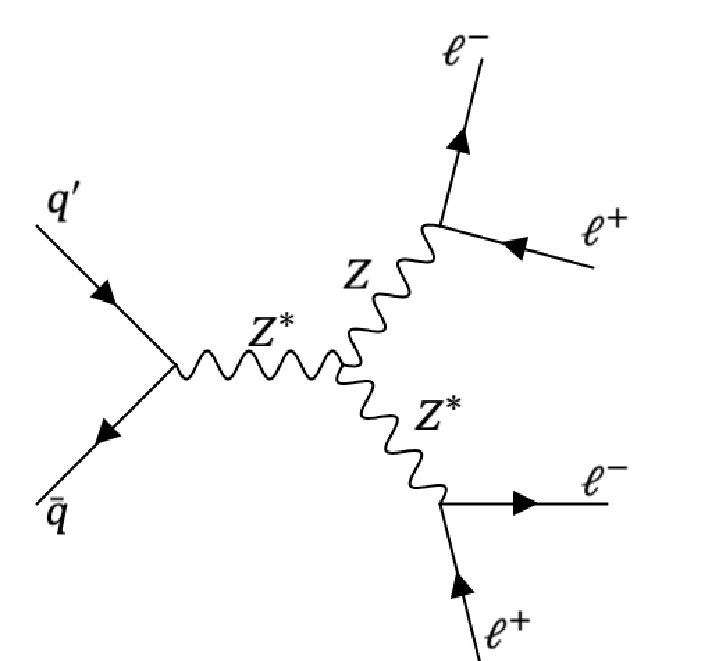
\includegraphics[width=0.4\textwidth]{figures/VH/qq_zz1.pdf}
    }
    \caption{Feynman diagrams for the two leading prompt backgrounds, $WZ$ and $ZZ$.}\label{fig:vh_wh_leading_prompt_bkg}
\end{figure}

Backgrounds in this analysis are estimated using several different methods. The first background category includes prompt processes such as $ZZ$, $VVV$ (not including $WWW$), $ttV$, and $tZ$, where all selected leptons originate from vector boson decays, and are estimated directly from MC simulation.

The second estimation strategy used involves a hybrid method using MC simulation, corrected with normalization factors (NFs) derived using a data-driven approach with a dedicated control region (CR) targeting a specific background. This method is detailed in Section~\ref{sec:vh_wh_wz_www_control_regions} and is used to estimate the $WZ/W\gamma^{*}$ and $WWW$ backgrounds, which are two of the dominant prompt backgrounds in the SRs.

The final background category consists of events with one non-prompt lepton originating from processes such as $Z+$jets, $Z+\gamma$, and $t\bar{t}$. The production of events with a non-prompt lepton is poorly modeled in both rate and shape by MC simulation and is therefore estimated using the data-driven techniques described in Section~\ref{sec:vh_wh_fake_lepton_estimation}. The leading non-prompt backgrounds are illustrated in Figure~\ref{fig:vh_wh_leading_nonprompt_bkg}. None of these processes produce three prompt leptons in the final state, instead, they enter the signal region through other mechanisms.

For $Z$+jets events, the final state contains a $Z$ boson and a quark (most often a $b$-quark). The $b$-quark hadronizes, and a lepton from the resulting decay chain is reconstructed. In the $Z+\gamma$ case, the photon is not from genuine $Z+\gamma$ production, but rather from final-state radiation (FSR) when a lepton from the $Z\to\ell^+\ell^-$ decay emits a photon. For the \ttbar{} process, both top quarks decay into a $W$ boson and a $b$-quark, where both $W$ bosons decay leptonically, and an additional lepton from a $b$-quark decay is reconstructed in the event.

\begin{figure}[htp]
    \centering
    \subfloat[$Z+$jets]{
        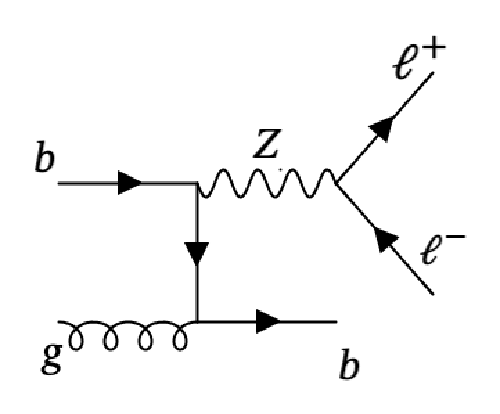
\includegraphics[width=0.32\textwidth]{figures/VH/z+jets.pdf}
    }
    \subfloat[$Z+\gamma$]{
        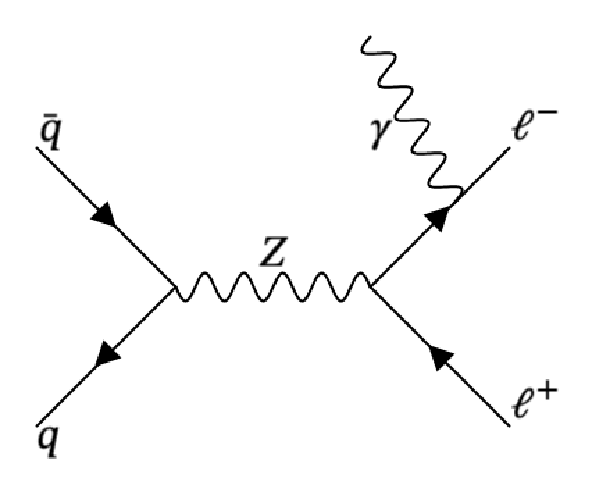
\includegraphics[width=0.32\textwidth]{figures/VH/zgamma.pdf}
    }
    \subfloat[\ttbar{}]{
        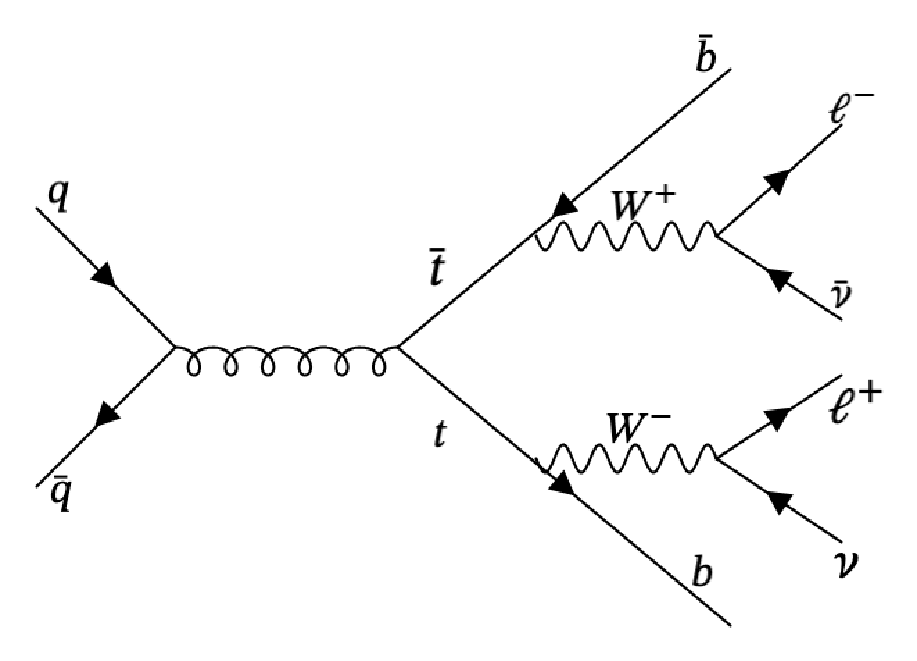
\includegraphics[width=0.32\textwidth]{figures/VH/ttbar.pdf}
    }\caption{Feynman diagrams for the three processes with non-prompt lepton contributions in the SR, $Z+$jets, $Z+\gamma$, and \ttbar{}}\label{fig:vh_wh_leading_nonprompt_bkg}
\end{figure}

Dedicated artificial neural networks are used in this analysis to enhance sensitivity with respect to a purely cut-based analysis. The \zdom{} and \zdep{} channels have different neural networks and their trainings are explained in detail in Section~\ref{sec:vh_wh_nn_training}. 

In the plots shown throughout this chapter, and the rest of this thesis that are directly related to the \wh{} analysis, the signal is represented as three entries in the legends. These entries are titled ``$WH$, Bin 1'', ``$WH$, Bin 2'', and ``$WH$, Bin 3'', corresponding to the different \ptv{} bins of the \wh{} process. Bin 1 is defined as $\ptv{} < 75$~GeV, Bin 2 as $75 \leq \ptv{} < 150$~GeV, and Bin 3 as $\ptv{} \geq 150$~GeV. Additionally, all uncertainties included in the plots include both statistical and systematic components, unless otherwise noted.

% \begin{table}
%     \centering
%     \begin{tabular}{c|c}
%         \hline
%         \textbf{Process} & \textbf{Cross section (pb)} \\
%         \hline\hline
%         $Z+\mathrm{jets}$ & $2.3\times10^{3}$ \\
%         $Z+\gamma$        & $1.0\times10^{2}$ \\
%         $t\bar{t}$        & $8.6\times10^{1}$ \\
%         $WZ$              & $4.8\times10^{0}$ \\
%         $ZZ$              & $1.3\times10^{0}$ \\
%         % $t\bar{t}W$       & $6.5\times10^{-1}$ \\
%         $WWW$             & $7.6\times10^{-3}$ \\
%         $W^{+}H$          & $6.8\times10^{-3}$ \\
%         $W^{-}H$          & $4.3\times10^{-3}$ \\
%         \hline
%     \end{tabular}
% \end{table}